 \documentclass[a4paper,10pt]{article}
 \usepackage{tikz}
 \usepackage{fullpage}
 \usetikzlibrary{positioning,shadows,arrows,trees,shapes,fit}
 \begin{document}
 \begin{figure}
 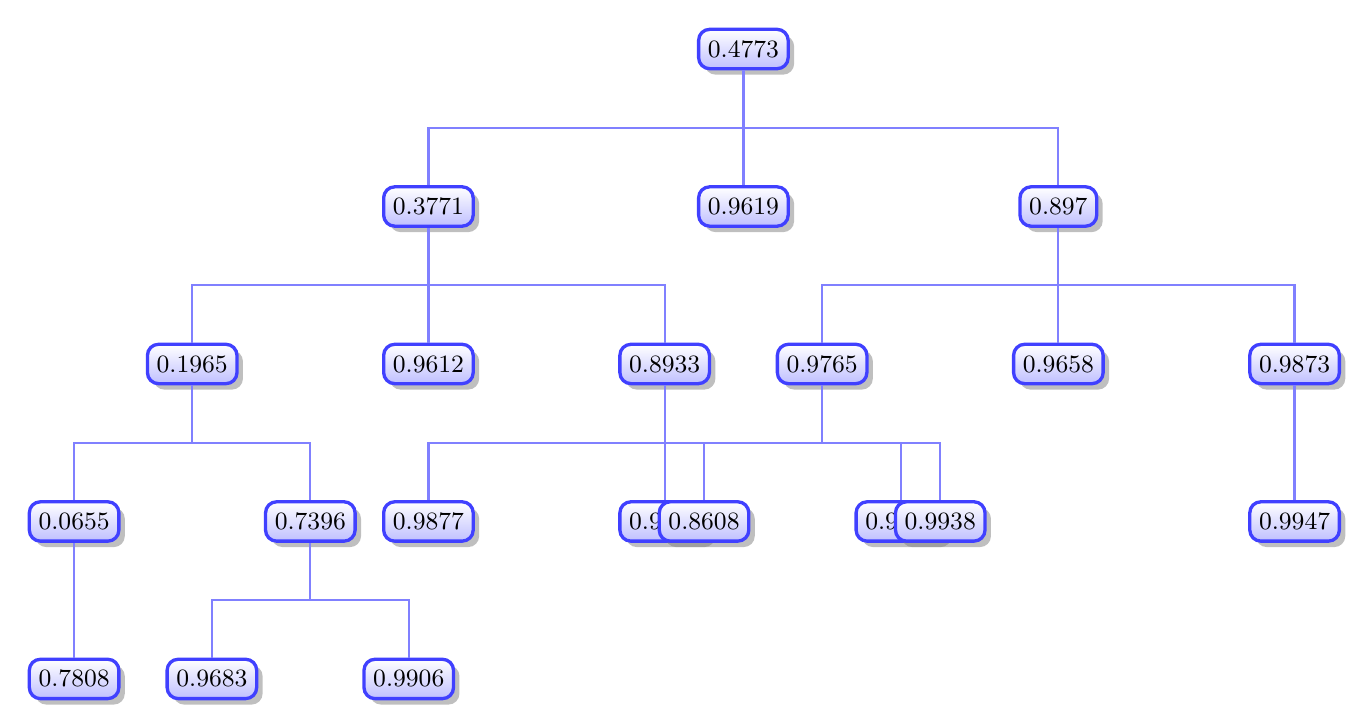
\begin{tikzpicture}
 [font=\small, edge from parent fork down, 
 every node/.style={top color=white, bottom color=blue!25, 
 	rectangle,rounded corners, minimum size=5mm, draw=blue!75,
	very thick, drop shadow, align=center},
 edge from parent/.style={draw=blue!50,thick},
 level 1/.style={sibling distance=4cm},
 level 2/.style={sibling distance=3cm}, 
 level 3/.style={sibling distance=3cm}, 
 level 4/.style={sibling distance=2.5cm}, 
 level 5/.style={sibling distance=2.5cm}, 
 level 6/.style={sibling distance=2cm}, 
 level 7/.style={sibling distance=2cm}, 
 level 8/.style={sibling distance=2cm}, 
 level distance=2cm,
 ]
\node {0.4773} %root
child { node {0.3771}  
child { node {0.1965}  
child { node {0.0655}  
child { node {0.7808}  
 }
 }
child { node {0.7396}  
child { node {0.9683}  
 }
child { node {0.9906}  
 }
 }
 }
child { node {0.9612}  
 }
child { node {0.8933}  
child { node {0.9877}  
 }
child { node {0.9918}  
 }
child { node {0.9946}  
 }
 }
 }
child { node {0.9619}  
 }
child { node {0.897}  
child { node {0.9765}  
child { node {0.8608}  
 }
child { node {0.9938}  
 }
 }
child { node {0.9658}  
 }
child { node {0.9873}  
child { node {0.9947}  
 }
 }
 }
;\end{tikzpicture} 
 \caption{Training plot }  \end{figure}
\end{document} 
